%\newcommand{\full}[1]{#1} \newcommand{\proce}[1]{}
\newcommand{\full}[1]{} \newcommand{\proce}[1]{#1}
\documentclass{beamer}%[handout]
\usepackage[utf8]{inputenc}
\usepackage{amsmath}
\usepackage{amssymb}					
\usepackage{mathdots}
\usepackage{tikz}
\usetikzlibrary{shapes,decorations.pathreplacing,calc,shapes.callouts,decorations.pathmorphing}

\usepackage[normalem]{ulem}
\newcommand{\tikzmark}[1]{\tikz[overlay,remember picture] \node (#1) {};}

\renewcommand{\vec}[1]{\mathbf{#1}}

\usepackage{listings}
\usepackage{algorithm}
\usepackage{algorithmic}
\usepackage{dsfont}
\definecolor{dunkelgrau}{rgb}{0.8,0.8,0.8}
\definecolor{hellgrau}{rgb}{0.95,0.95,0.95}
\definecolor{myred}{rgb}{0.7,0.0627,0.1627}
\definecolor{myblue}{rgb}{.222,.62,.99}
\definecolor{lightblue}{rgb}{.222,.62,.9}
\definecolor{mygreen}{rgb}{.222,.62,.49}
\definecolor{lightgreen}{rgb}{.222,.6,.45}

\definecolor{mg}{rgb}{0.008,0.717,0.35}
\definecolor{LightCyan}{rgb}{0.88,1,1}
\renewcommand{\arraystretch}{1.2}
\usepackage{colortbl}
\usepackage{enumerate}
\usepackage{float}
\usepackage{algorithmic}
%\usetheme{umbc4}
%\usecolortheme{beaver}
\useinnertheme[shadow=true]{rounded}
\setbeamertemplate{navigation symbols}{}

%\beamersetuncovermixins{\opaqueness<1>{55}}{\opaqueness<2->{4}}%text light
%%%%%%%%%%%%%%%%%%%%%%%%%%%%%%%%%%%%%%%%%%%%%%%%%%%%%%%%%%%
%%%%%%%%%%%%%%%%%%%%%%
\newcommand{\mr}[1]{\color{myred}{#1}}
\newcommand{\mb}[1]{\color{myblue}{#1}}
\newcommand{\mg}[1]{\color{mg}{#1}}
\newcommand{\Ot}{{\cal \tilde O}}
\newcommand{\Ocal}{{\cal O}}
\newcommand{\LL}{\mathbb{L}}

\newcommand{\K}{\mathbb{K}}
\newcommand{\F}{\mathbb{F}}
\newcommand{\R}{\mathbb{R}}
\newcommand{\ba}{\mathbf{a}}
\newcommand{\la}{\leftarrow}
\newcommand{\ra}{\rightarrow}
\newcommand{\e}{\varepsilon}
\newcommand{\w}{\omega}
\newcommand{\KK}{\mathbb{K}}
\newcommand{\Z}{\mathbb{Z}}
\newcommand{\CC}{\mathbb{C}}
\newcommand{\vol}{\text{vol}}
\newcommand{\Ls}{\mathcal{L}}
\newcommand{\Exp}[1]{\mathbb{E}{(#1)}}
\newcommand{\norm}[1]{ \Vert{ #1 \Vert }}
\newcommand{\done}{\item[\Large \color{mygreen}\checkmark]}
\newcommand{\notdone}{\item[\Large \color{myred}$\times$]}
\newcommand{\Ball}{\text{Ball}}
\usetikzlibrary{arrows,positioning} 
\usetikzlibrary{calc,shadows,through}
\tikzstyle{message} = [draw, fill=black!05, rectangle,minimum height=1.7em, minimum width=8em, drop shadow,thick]

\tikzstyle{to} = [->,thick]
\newcommand{\atmid}[3]{
ÊÊ\coordinate (mid) at ($0.5*(#1.center) + 0.5*(#2.center)$);
ÊÊ\node at (mid) {#3};
}
\def \myvskip {\vspace{.3cm}}
\def \myskip {\hskip 1em}
    \setbeamercolor{upyellow}{fg=black,bg=yellow!20}
    \setbeamercolor{lowyellow}{fg=black,bg=yellow!40}
\setbeamercolor{lowgreen}{fg=black,bg=lightgreen!10}
\setbeamercolor{block body example}{bg=mygreen!10}%bg=background, fg= foreground
\setbeamercolor{block title example}{bg=blue!10}%bg=background, fg= foreground
\setbeamercolor{block body}{bg=yellow!10}%bg=background, fg= foreground
\setbeamercolor{block title}{bg=blue!10}%bg=background, fg= foreground


\title{Comparing the Jacobi Method and LLL lattice reduction algorithms for cryptographic applications}
 
\subtitle{IN  Bachelor Semester Project}

\institute[EPFL]{
  
\includegraphics[scale=.065]{pics/epfl-logo.png}
}

\author{Frederic ~Jacobs}
  
\date{Fall 2014}
 
\begin{document}

\frame{\titlepage}

\AtBeginSection[]{
     \frame{
         \frametitle{Overview}
         \tableofcontents[currentsection]
     }
}

\section{Reminders about lattices}

\frame{\frametitle{Lattice}
\center
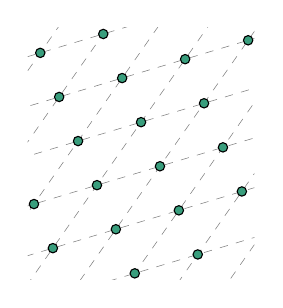
\begin{tikzpicture}[scale=0.4]
    \coordinate (Origin)   at (0,0);
    \coordinate (XAxisMin) at (-3,0);
    \coordinate (XAxisMax) at (5,0);
    \coordinate (YAxisMin) at (0,-2);
    \coordinate (YAxisMax) at (0,5);
%   \draw [thin, gray,-latex] (XAxisMin) -- (XAxisMax);% Draw x axis
%    \draw [thin, gray,-latex] (YAxisMin) -- (YAxisMax);% Draw y axis

    \clip (-2.2,-3) rectangle (5cm,5cm); % Clips the picture...
    \pgftransformcm{1}{0.3}{0.7}{1}{\pgfpoint{0cm}{0cm}}
          
    \draw[style=help lines,dashed] (-14,-14) grid[step=2cm] (14,14); % Draws a grid in the new coordinates.
%    \filldraw[fill=gray, fill opacity=0.3] (0,0) rectangle (2,2);                % Puts the shaded rectangle
%	 \node (b) at (1.6,-0.5) {$b_1$} ;
%   \node (b) at (-0.7,1.7) {$b_2$} ;    
   
    \foreach \x in {-14,-12,...,14}{% Two indices running over each
      \foreach \y in {-14,-12,...,14}{% node on the grid we have drawn 
        \node[draw,circle,inner sep=1.2pt,fill=mygreen] at (\x,\y) {};
            % Places a dot at those points
      }
    }
  %  \node[draw,circle,inner sep=11pt] at (0,0) {};
      %\draw [thin, gray,-latex] (0,0) -- (3.5,-1) node [below, node distance =0.2cm] {} ;
   %\draw [thin, gray,-latex] (0,0) -- (-2,2) node [below, node distance =0.2cm] {} ;
  % \node (b) at (-2,1.8) {$v$} ;
  
    % \draw [thin, gray,-latex] (2.4,0.1) -- (0.9,1.5)node [below left] {$e$} ;
   % \path [line] (0,0) -- (0,3.9);
%    \draw [ultra thick,-latex,red] (Origin)
%        -- (Bone) node [above left] {$b_1$};
%    \draw [ultra thick,-latex,red] (Origin)
%        -- (Btwo) node [below right] {$b_2$};
%    \draw [ultra thick,-latex,red] (Origin)
%        -- ($(Bone)+(Btwo)$) node [below right] {$b_1+b_2$};
%    \draw [ultra thick,-latex,red] (Origin)
%        -- ($2*(Bone)+(Btwo)$) node [above left] {2$b_1+b_2$};
%    \filldraw[fill=gray, fill opacity=0.3, draw=black] (Origin)
%        rectangle ($2*(Bone)+(Btwo)$);
%    %\draw [thin,-latex,red, fill=gray, fill opacity=0.3] (0,0)
        % -- ($2*(0,2)+(2,-2)$)
        % -- ($3*(0,2)+2*(2,-2)$) -- ($(0,2)+(2,-2)$) -- cycle;
  \end{tikzpicture}\hspace{2cm}
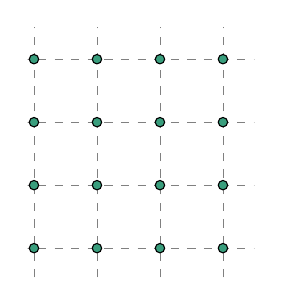
\begin{tikzpicture}[scale=0.4]
    \coordinate (Origin)   at (0,0);
    \coordinate (XAxisMin) at (-3,0);
    \coordinate (XAxisMax) at (5,0);
    \coordinate (YAxisMin) at (0,-2);
    \coordinate (YAxisMax) at (0,5);
%   \draw [thin, gray,-latex] (XAxisMin) -- (XAxisMax);% Draw x axis
%    \draw [thin, gray,-latex] (YAxisMin) -- (YAxisMax);% Draw y axis

    \clip (-2.2,-3) rectangle (5cm,5cm); % Clips the picture...
   % \pgftransformcm{1}{0.3}{0.7}{1}{\pgfpoint{0cm}{0cm}}
          
    \draw[style=help lines,dashed] (-14,-14) grid[step=2cm] (14,14); % Draws a grid in the new coordinates.
%    \filldraw[fill=gray, fill opacity=0.3] (0,0) rectangle (2,2);                % Puts the shaded rectangle
%	 \node (b) at (1.6,-0.5) {$b_1$} ;
%   \node (b) at (-0.7,1.7) {$b_2$} ;    
   
    \foreach \x in {-14,-12,...,14}{% Two indices running over each
      \foreach \y in {-14,-12,...,14}{% node on the grid we have drawn 
        \node[draw,circle,inner sep=1.2pt,fill=mygreen] at (\x,\y) {};
            % Places a dot at those points
      }
    }
  %  \node[draw,circle,inner sep=11pt] at (0,0) {};
      %\draw [thin, gray,-latex] (0,0) -- (3.5,-1) node [below, node distance =0.2cm] {} ;
   %\draw [thin, gray,-latex] (0,0) -- (-2,2) node [below, node distance =0.2cm] {} ;
  % \node (b) at (-2,1.8) {$v$} ;
  
    % \draw [thin, gray,-latex] (2.4,0.1) -- (0.9,1.5)node [below left] {$e$} ;
   % \path [line] (0,0) -- (0,3.9);
%    \draw [ultra thick,-latex,red] (Origin)
%        -- (Bone) node [above left] {$b_1$};
%    \draw [ultra thick,-latex,red] (Origin)
%        -- (Btwo) node [below right] {$b_2$};
%    \draw [ultra thick,-latex,red] (Origin)
%        -- ($(Bone)+(Btwo)$) node [below right] {$b_1+b_2$};
%    \draw [ultra thick,-latex,red] (Origin)
%        -- ($2*(Bone)+(Btwo)$) node [above left] {2$b_1+b_2$};
%    \filldraw[fill=gray, fill opacity=0.3, draw=black] (Origin)
%        rectangle ($2*(Bone)+(Btwo)$);
%    %\draw [thin,-latex,red, fill=gray, fill opacity=0.3] (0,0)
        % -- ($2*(0,2)+(2,-2)$)
        % -- ($3*(0,2)+2*(2,-2)$) -- ($(0,2)+(2,-2)$) -- cycle;
  \end{tikzpicture}
 	\begin{itemize}
 	\item Discrete, additive subgroup of $\R^m$
 	\item Intersecting points of an infinite regular $n$-dimensional grid in $\R^m$    
	\end{itemize}
}

\frame{\frametitle{Lattice}
\begin{columns}[]
 \begin{column}{0.3\textwidth}
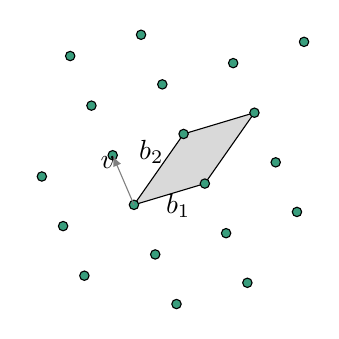
\begin{tikzpicture}[scale=0.45]
    \coordinate (Origin)   at (0,0);
    \coordinate (XAxisMin) at (-3,0);
    \coordinate (XAxisMax) at (5,0);
    \coordinate (YAxisMin) at (0,-2);
    \coordinate (YAxisMax) at (0,5);
 %  \draw [thin, gray,-latex] (XAxisMin) -- (XAxisMax);% Draw x axis
  %  \draw [thin, gray,-latex] (YAxisMin) -- (YAxisMax);% Draw y axis

    \clip (-3,-3) rectangle (5cm,5cm); % Clips the picture...
    \pgftransformcm{1}{0.3}{0.7}{1}{\pgfpoint{0cm}{0cm}}
          % This is actually the transformation matrix entries that
          % gives the slanted unit vectors. You might check it on
           % MATLAB etc. . I got it by guessing.
    %\coordinate (Bone) at (0,2);
    %\coordinate (Btwo) at (2,-2);
%    \draw[style=help lines,dashed] (-14,-14) grid[step=2cm] (14,14);
%          % Draws a grid in the new coordinates.
          \filldraw[fill=gray, fill opacity=0.3] (0,0) rectangle (2,2);
  
   \foreach \x in {-14,-12,...,14}{% Two indices running over each
      \foreach \y in {-14,-12,...,14}{% node on the grid we have drawn 
        \node[draw,circle,inner sep=1.2pt,fill=mygreen] at (\x,\y) {};  }}
  
   \draw [thin, gray,-latex] (0,0) -- (-2,2) node [below, node distance =0.2cm] {} ;
   \node (b) at (-2,1.8) {$v$} ;
   \node (b) at (1.6,-0.5) {$b_1$} ;
   \node (b) at (-0.7,1.7) {$b_2$} ;  
    % \draw [thin, gray,-latex] (2.4,0.1) -- (0.9,1.5)node [below left] {$e$} ;
   % \path [line] (0,0) -- (0,3.9);
%    \draw [ultra thick,-latex,red] (Origin)
%        -- (Bone) node [above left] {$b_1$};
%    \draw [ultra thick,-latex,red] (Origin)
%        -- (Btwo) node [below right] {$b_2$};
%    \draw [ultra thick,-latex,red] (Origin)
%        -- ($(Bone)+(Btwo)$) node [below right] {$b_1+b_2$};
%    \draw [ultra thick,-latex,red] (Origin)
%        -- ($2*(Bone)+(Btwo)$) node [above left] {2$b_1+b_2$};
%    \filldraw[fill=gray, fill opacity=0.3, draw=black] (Origin)
%        rectangle ($2*(Bone)+(Btwo)$);
%    %\draw [thin,-latex,red, fill=gray, fill opacity=0.3] (0,0)
        % -- ($2*(0,2)+(2,-2)$)
        % -- ($3*(0,2)+2*(2,-2)$) -- ($(0,2)+(2,-2)$) -- cycle;
  \end{tikzpicture}
 \end{column}
 \begin{column}{0.7\textwidth}
 	\begin{itemize}
 	\item Set $B=\{\vec{b}_1,..,\vec{b}_n\} \subset\R^m$, \\$\vec{b}_i$ are linearly independent
 	\item Full-rank lattices: $n = m$
 	\begin{block}{}
	Set of \alert{integer} linear combinations
 	$$\text{Lattice }\Ls = \sum_i \alert{\Z}\cdot \vec{b}_i $$
 	\end{block}
	\item $B$ is called a basis of $\Ls$, it is not unique
	\item the volume of a full-rank lattice is given by $\text{vol}(\Ls) = |det(B)|$
	\end{itemize}
 \end{column}
\end{columns}
}

\frame{
\frametitle{Random Lattice}

We say that a lattice is a random lattice $L$ of prime volume $P$ if under HNF form its basis matrix $B$ has the following properties:

\begin{itemize}
\item the diagonal has 1 for all it's entries except one position that is set to a prime number $P$. Hence, the $\det(B)$ is prime.
\item All row entries of the matrix right to the position that is set to $P$ are smaller than $P$ in absolute value.
\end{itemize}

Without loss of generality, we hence restrict tests to random lattices of volume $P$ whose basis in HNF form is as follows:
$$\begin{array}{ccccc}
P & \vec{a_2} & \dots & \vec{a_{m}}\\
 & 1&   & \\ 
& & \ddots & \\ 
& & &1 
\end{array}$$
where $a_i \in \mathbb{Z}/ P\mathbb{Z}$.
}

\frame{
\frametitle{Almost Orthogonal Lattice Bases}

We define an \emph{almost orthogonal lattice basis} $M$ of dimension $n$ and of bit length $k$ as an $n \times n$ square matrix whose entries are $k$-bit integers picked at random.

}

\frame{
\frametitle{Gram Schmidt orthogonalisation - GSO}
\begin{itemize}
\item Basis $B = (\vec{b}_1, \ldots, \vec{b}_n)$
\item Compute GSO of $B$:\\
 $\vec{b}_1^* = \vec{b}_1$\\
 $\vec{b}_2^* = \vec{b}_2 - \frac{\langle b_2, b_1^*\rangle}{\|\vec{b}_1\|^2} \vec{b}_1$\\
  $\vec{b}_3^* = \vec{b}_3 - \frac{\langle b_3, b_1^*\rangle}{\|b_1\|^2} \vec{b}^*_1- \frac{\langle b_3, b_2^*\rangle}{\|b_2^*\|^2} \vec{b}_2^*$\\
  $\ldots$
  
  \vspace{.3cm}
%\item Obtain $\pi_i(b_i) = b_i^*$ as\\
\item In general 
 $$\vec{b}_i^* = \vec{b}_i - \sum_{j<i}  \mu_{ij}  \vec{b}_j^* \text{ where }\mu_{ij} := \frac {\langle b_i, b_j^*\rangle} { \|b_j^*\|^2 }$$
\end{itemize}
}

\frame{
\frametitle{The LLL Algorithm}
\begin{itemize}
\item First polynomial-time reduction algorithm to be introduced outputting a nearly orthogonal basis
\item LLL and BKZ 2.0 are the two reduction algorithms that are used in practice for applications in cryptology and digital signal processing (MIMO)
\end{itemize}
}

\frame{
\frametitle{$\delta$-LLL Reduced}

\begin{block}{$\delta$-LLL Reduced}
Ordered basis $b_1, \ldots, b_n \in \R^m$ of $\Ls$, parameter $\delta\in (1/4, 1]$, s.t. $\forall i,j:$
\begin{itemize}
\item $| \mu_{i,j}| \leq \frac{1}{2} $ for $1 \leq j < i \leq n$\\
\pause
\item $\forall (\vec{b_i, b_{i+1}})$, we have $(\delta - \mu^2_{i+1,i}) \|\vec{b}^{\star}_{i}\|^2 \leq \| \vec{b}^{\star}_{i+1} \|^2$
\end{itemize}
\end{block}
\begin{columns}[]
\begin{column}{0.5\textwidth}
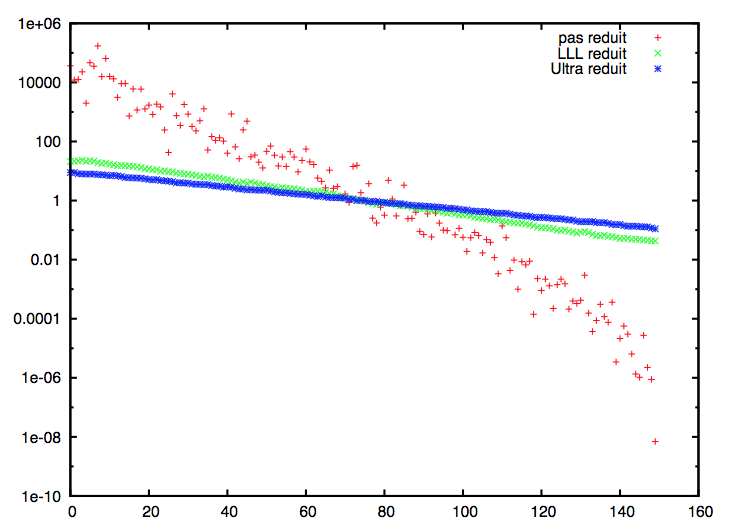
\includegraphics[scale=.2]{pics/GSO.png}
\end{column}
\end{columns}
}
    
\section{Jacobi Method for lattice reduction}

\frame{
\frametitle{Jacobi method for lattice reduction}
\begin{itemize}
\item May 2012: Sanzheng Qiao publishes generic Jacobi paper\cite{originalJacobiMethodLatticeBasisReduction}
\item June 2012: Complexity analysis \cite{complexityAnalysisOfJacobiMethod}
\item July 2013: An Enhanced Jacobi Method for Lattice-Reduction-Aided MIMO Detection\cite{enhancedJacobi}
\item January 2014: A Hybrid Method for Lattice Basis Reduction\cite{tian2014hybrid}
\item Summer 2014: A Fast Jacobi-Type Method for Lattice Basis Reduction\cite{fastJacobi}
\end{itemize}
}

\frame{
\frametitle{Euclid's centered algorithm}
\begin{algorithm}[H]
\caption{Euclid's centered algorithm}
\label{euclidsAlgorithm}
\begin{algorithmic}[1]
\REQUIRE $(n, m) \in \mathbb{Z}^2$
\ENSURE  gcd($n,m$)

\IF{$|n| < |m|$} \STATE{swap $n$ and $m$} \ENDIF

\WHILE{$m \neq 0$} 
    \STATE{$r \leftarrow n - qm$ where $q = \lfloor \frac{n}{m} \rceil$} 
    \STATE{$n \leftarrow m$}
    \STATE{$m \leftarrow r$}
\ENDWHILE

\STATE{Output $n$}

\end{algorithmic}
\end{algorithm}
}


\frame{
\frametitle{Lagrange algorithm}
\begin{algorithm}[H]
\caption{Lagrange algorithm}
\label{lagrangeAlgorithm}
\begin{algorithmic}[1]
\REQUIRE Two basis ($\vec{b_1, b_2}$) vectors.
\ENSURE a Lagrange reduced reduced basis $(\vec{b_1, b_2})$

\IF{$\|\vec{b_1} \| < \| \vec{b_2} \| $} \STATE{swap $\vec{b_1}$ and $\vec{b_2}$} \ENDIF
\REPEAT \STATE{
$q = \lfloor \frac{ \langle \vec{b_1} \vec{b_2} \rangle }{\| \vec{b_2} \|^2} \rceil $\\
$r \leftarrow \vec{b_1} - q \vec{b_2}$\\
$\vec{b_1} \leftarrow \vec{b_2}$\\
$\vec{b_2} \leftarrow r$
} \UNTIL{$\| \vec{b_1} \| \leq \| \vec{b_2} \| $}

\end{algorithmic}
\end{algorithm}
}

\frame{
    \frametitle{The generic Jacobi Method}
    \begin{algorithm}[H]
\caption{Generic Jacobi Method}
\label{genericJacobiMethod}
\begin{algorithmic}
\REQUIRE a basis matrix ($\vec{b_1,...,b_n}$)
\ENSURE a generic-Jacobi reduced basis ($\vec{b_1,...,b_n}$)

\WHILE{not all pairs ($\vec{b_i,b_j}$) satisfy both generic-Jacobi reduction conditions}
    \FOR{$i = 1$ \TO $n-1$ }
        \FOR{$j = i + 1$ \TO $n$ }
            \STATE {$[\vec{b_i, b_j}]$} = \emph{Lagrange$(\vec{b_i, b_j})$}
        \ENDFOR
    \ENDFOR
\ENDWHILE

\end{algorithmic}
\end{algorithm}
}

\frame{
\frametitle{$\omega$-Lagrange reduced}
There are two conditions for a basis to be $\omega$-Lagrange-reduced.

\[
\begin{cases}
\lfloor g_{ij} / g_{ss} \rceil \leq 1, \\
\omega^2 g_{ll} \leq g_{ii} + g_{jj} - 2|g_{ij}|

\end{cases}
\]  where $1/\sqrt{3} \leq \omega < 1$ and $g_ij$ the entries of the Gram matrix $G$ at indexes ($i,j$).

}

\frame{
\frametitle{Iterative Lagrange}
\scalebox{0.80}{\begin{minipage}{\textwidth}
    \begin{algorithm}[H]
\caption{LagrangeIT}
\label{customLagrangeIT}
\begin{algorithmic}
\REQUIRE The matrices $G, Z$, a pair of indices $(i,j):i<j$ and a parameter $\omega$
\ENSURE  Updated $G, Z$ where one Lagrange iteration was performed on the $i$th and $j$th basis vectors. 

\STATE {$s \leftarrow i$}
\STATE {$l \leftarrow j$}

\IF{$g_{ii} > g_{jj}$}
    \STATE {$s \leftarrow j; l \leftarrow i$}
\ENDIF

\STATE{$q \leftarrow \lfloor \frac {g_{ij}}{g_{ss}} \rceil$}

\IF {Verify both $\omega$-Lagrange-reduced conditions}

\STATE{$\vec{z}_l -= q* \vec{z}_s$}
\STATE{$\vec{g}_l -= q* \vec{g}_s$}

\STATE{Updating entries of the Gram matrix}
\ENDIF

\end{algorithmic}
\end{algorithm}

\end{minipage}}
}

\frame{
    \frametitle{The Fast Jacobi method}
    \begin{algorithm}[H]
\caption{Fast-Jacobi Reduction}
\label{jacobiVariantReduction}
\begin{algorithmic}
\REQUIRE a basis matrix ($\vec{B = b_1,...,b_n}$) and $\omega$
\ENSURE a reduced basis ($\vec{b_1,...,b_n}$) where each pair of vectors is $\omega$-Lagrange reduced
\STATE{$G = B^T B$, $Z = I_n$}
\WHILE{LagrangeIT method reduced the basis vectors}
    \FOR{$i = 1$ \TO $n-1$ }
        \FOR{$j = i + 1$ \TO $n$ }
            \STATE {$[G, Z]$} = \emph{LagrangeIT$(G,Z,i,j,\omega)$}
        \ENDFOR
    \ENDFOR
\ENDWHILE

\end{algorithmic}
\end{algorithm}
}

\section{Experimental results}

\frame{
\frametitle{Our Implementation}

\begin{itemize}
\item Generic and Fast-Jacobi implemented
\item Written in C++ with newNTL
\item ZZ and double implementations
\item Benchmarked against FPLLL ($\delta = 0.99$)
\end{itemize}

}

\frame{
\frametitle{Reduction quality indicators}
\begin{block}{Orthogonality Defect}
The \emph{orthogonality defect} of a basis $\vec{b_1},\vec{b_2},...,\vec{b_n}$ of a lattice $L$ is defined by:
\[
    \text{OrthDefect}(L) :=  \sqrt[n]{\frac{\displaystyle\prod^{n}_{i=1} \|\vec{b_i}\| }{\det(L)}}
\]
\end{block}

\begin{block}{Hermite Factor}
The \emph{Hermite factor} of basis vectors $\vec{b_1}, \vec{b_2},...,\vec{b_n}$ of a lattice $L$ is defined by

\[
    \text{HF}(L) := \frac{\|\vec{b_1}\|}{\sqrt[n]{\det(L)}}
\]
\end{block}
}

\frame{
\frametitle{Almost orthogonal basis, $\omega=0.6$}
\begin{center}
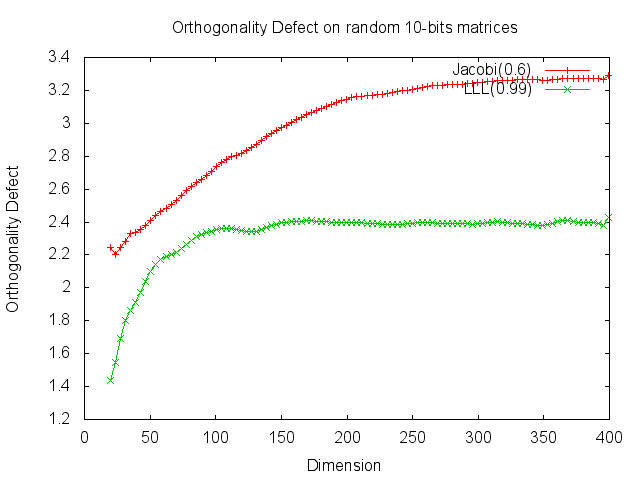
\includegraphics[width=\textwidth]{results-graphs/random-matrix-omega-06defect.png}
\end{center}
}

\frame{
\frametitle{Almost orthogonal basis, $\omega=0.99$}
\begin{center}
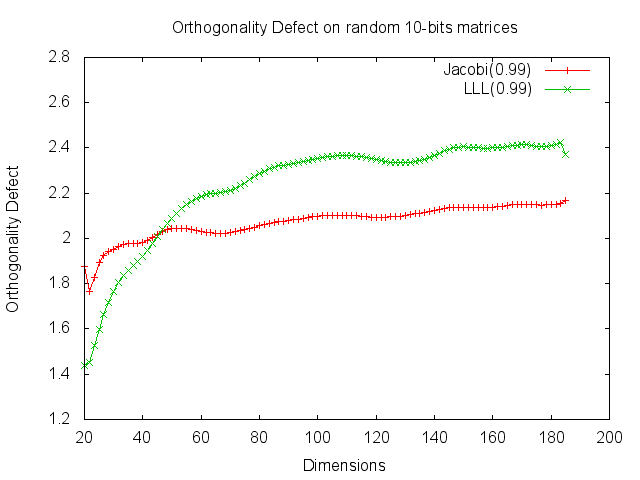
\includegraphics[width=\textwidth]{results-graphs/random-matrix-omega-09defect.png}
\end{center}
}

\frame{
\frametitle{Average number of inner loops by $\omega$}
\begin{center}
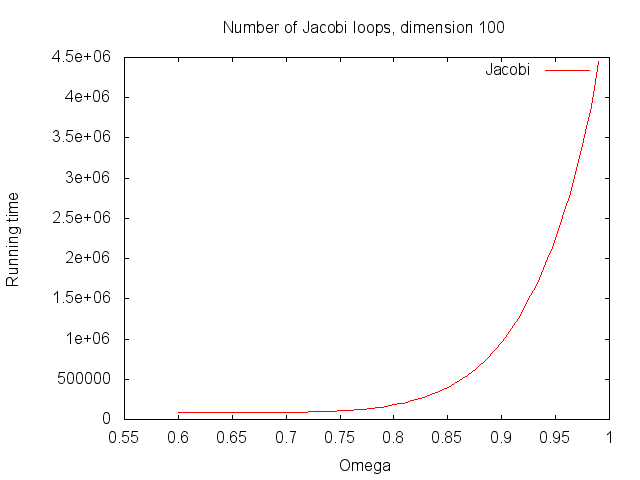
\includegraphics[width=\textwidth]{results-graphs/loops.png}
\end{center}
}

\frame{
\frametitle{Note on running time depending on Omega}
\begin{center}
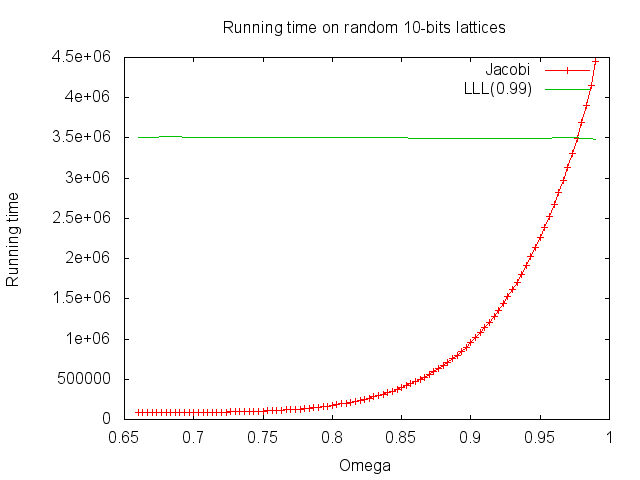
\includegraphics[width=\textwidth]{results-graphs/runningTime.png}
\end{center}
}

\frame{
\frametitle{Jacobi after LLL}
\begin{center}
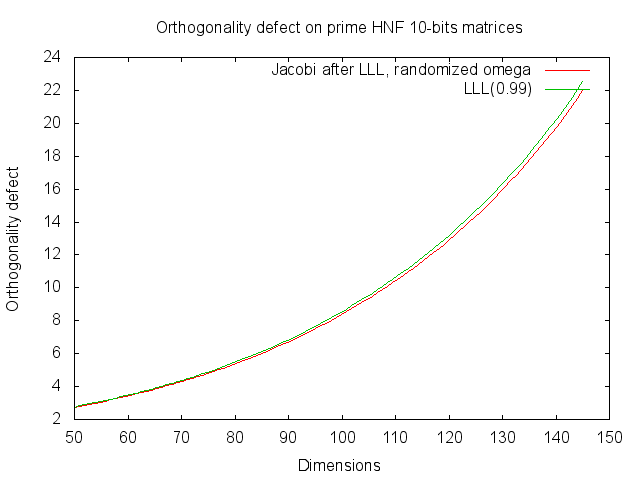
\includegraphics[width=\textwidth]{results-graphs/LLLThenJacobi/defect.png}
\end{center}
}

\frame{
\frametitle{Jacobi after LLL}
\begin{center}
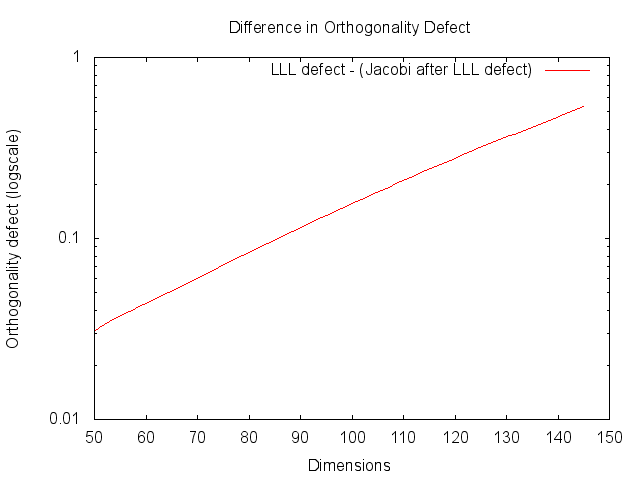
\includegraphics[width=\textwidth]{results-graphs/LLLThenJacobi/defect-logscale-difference.png}
\end{center}
}

\frame{
\frametitle{Jacobi after LLL}
\begin{block}{Example of LLL-reduced basis but not Jacobi-reduced}

\[
B = \begin{bmatrix}
  \vec{b_1} \\
  \vec{b_2} \\
  \vec{b_3}
 \end{bmatrix} = \begin{bmatrix}
  0 & 2 & 0 \\
  0 & 1 & 2 \\
  2 & 0 & 0
 \end{bmatrix}
\]
\end{block}
}


\section{Acknowledgements and Bibliography}

\frame{
\frametitle{Acknowledgements}
Thanks LACAL, particularly Anja and Nicolas.
}

\frame[shrink=20]{
\frametitle{Bibliography}
\bibliographystyle{alpha}
\bibliography{references}
} 

\frame[plain]{
\vspace{3cm}
\begin{flushright}\Large
\cal{Thank you}
\end{flushright}
}

\end{document}
